\section{Timing pipeline components on Summit and Theta}

\subsection{Offloading Gray-Scott to GPU with Kokkos}

\begin{frame}[fragile]
  \frametitle{Offloading Gray-Scott to GPU with Kokkos}
  \begin{itemize}
  \item The original version of Gray-Scott runs on CPU using MPI
  \item To justify using Summit, Gray-Scott was accelerated with Kokkos
  \item The same code - one line change - can be used to offload to GPU on Summit or to use multithreading on Theta
  \end{itemize}

  {\tiny
    \begin{table}[H]
      \centering
      \begin{tabular}{|r||r|r|r|r||r|r|r|}
        \hline
	& CPU & CPU & CPU & CPU & GPU & GPU & GPU\\
        \hline
	MPI ranks & 1 & 8 & 21 & 42 & 1 & 3 & 6\\
        \hline
	compute/rank/iteration, ms & 199,972 & 23,743 & 9,911 & 4968 & 1,819 & 625 & 404\\
        \hline
	write/rank/iteration, ms & 7,597 & 3,414 & 531 & 335 & 7850 & 2887 & 1631\\
        \hline
      \end{tabular}
      \caption{L=512, summit}
      \label{kokkos_512_summit}
    \end{table}
  }
  
  \begin{itemize}
  \item To use Kokkos requires some bleeding edge compiler specifically built to offload to GPU, same applies to OpenMP GPU offloading
  \item I am using LLVM 9.0.0 on Summit
  \item On Theta, while I can build Kokkos version of Gray-Scott, I had some trouble compiling some other components of the pipeline.
    So for now I am using original version of Gray-Scott on Theta.
  \end{itemize}

\end{frame}


\subsection{Gantt chart on Theta}

\begin{frame}[fragile]
  \frametitle{Gantt chart on Theta}

  \begin{center}
    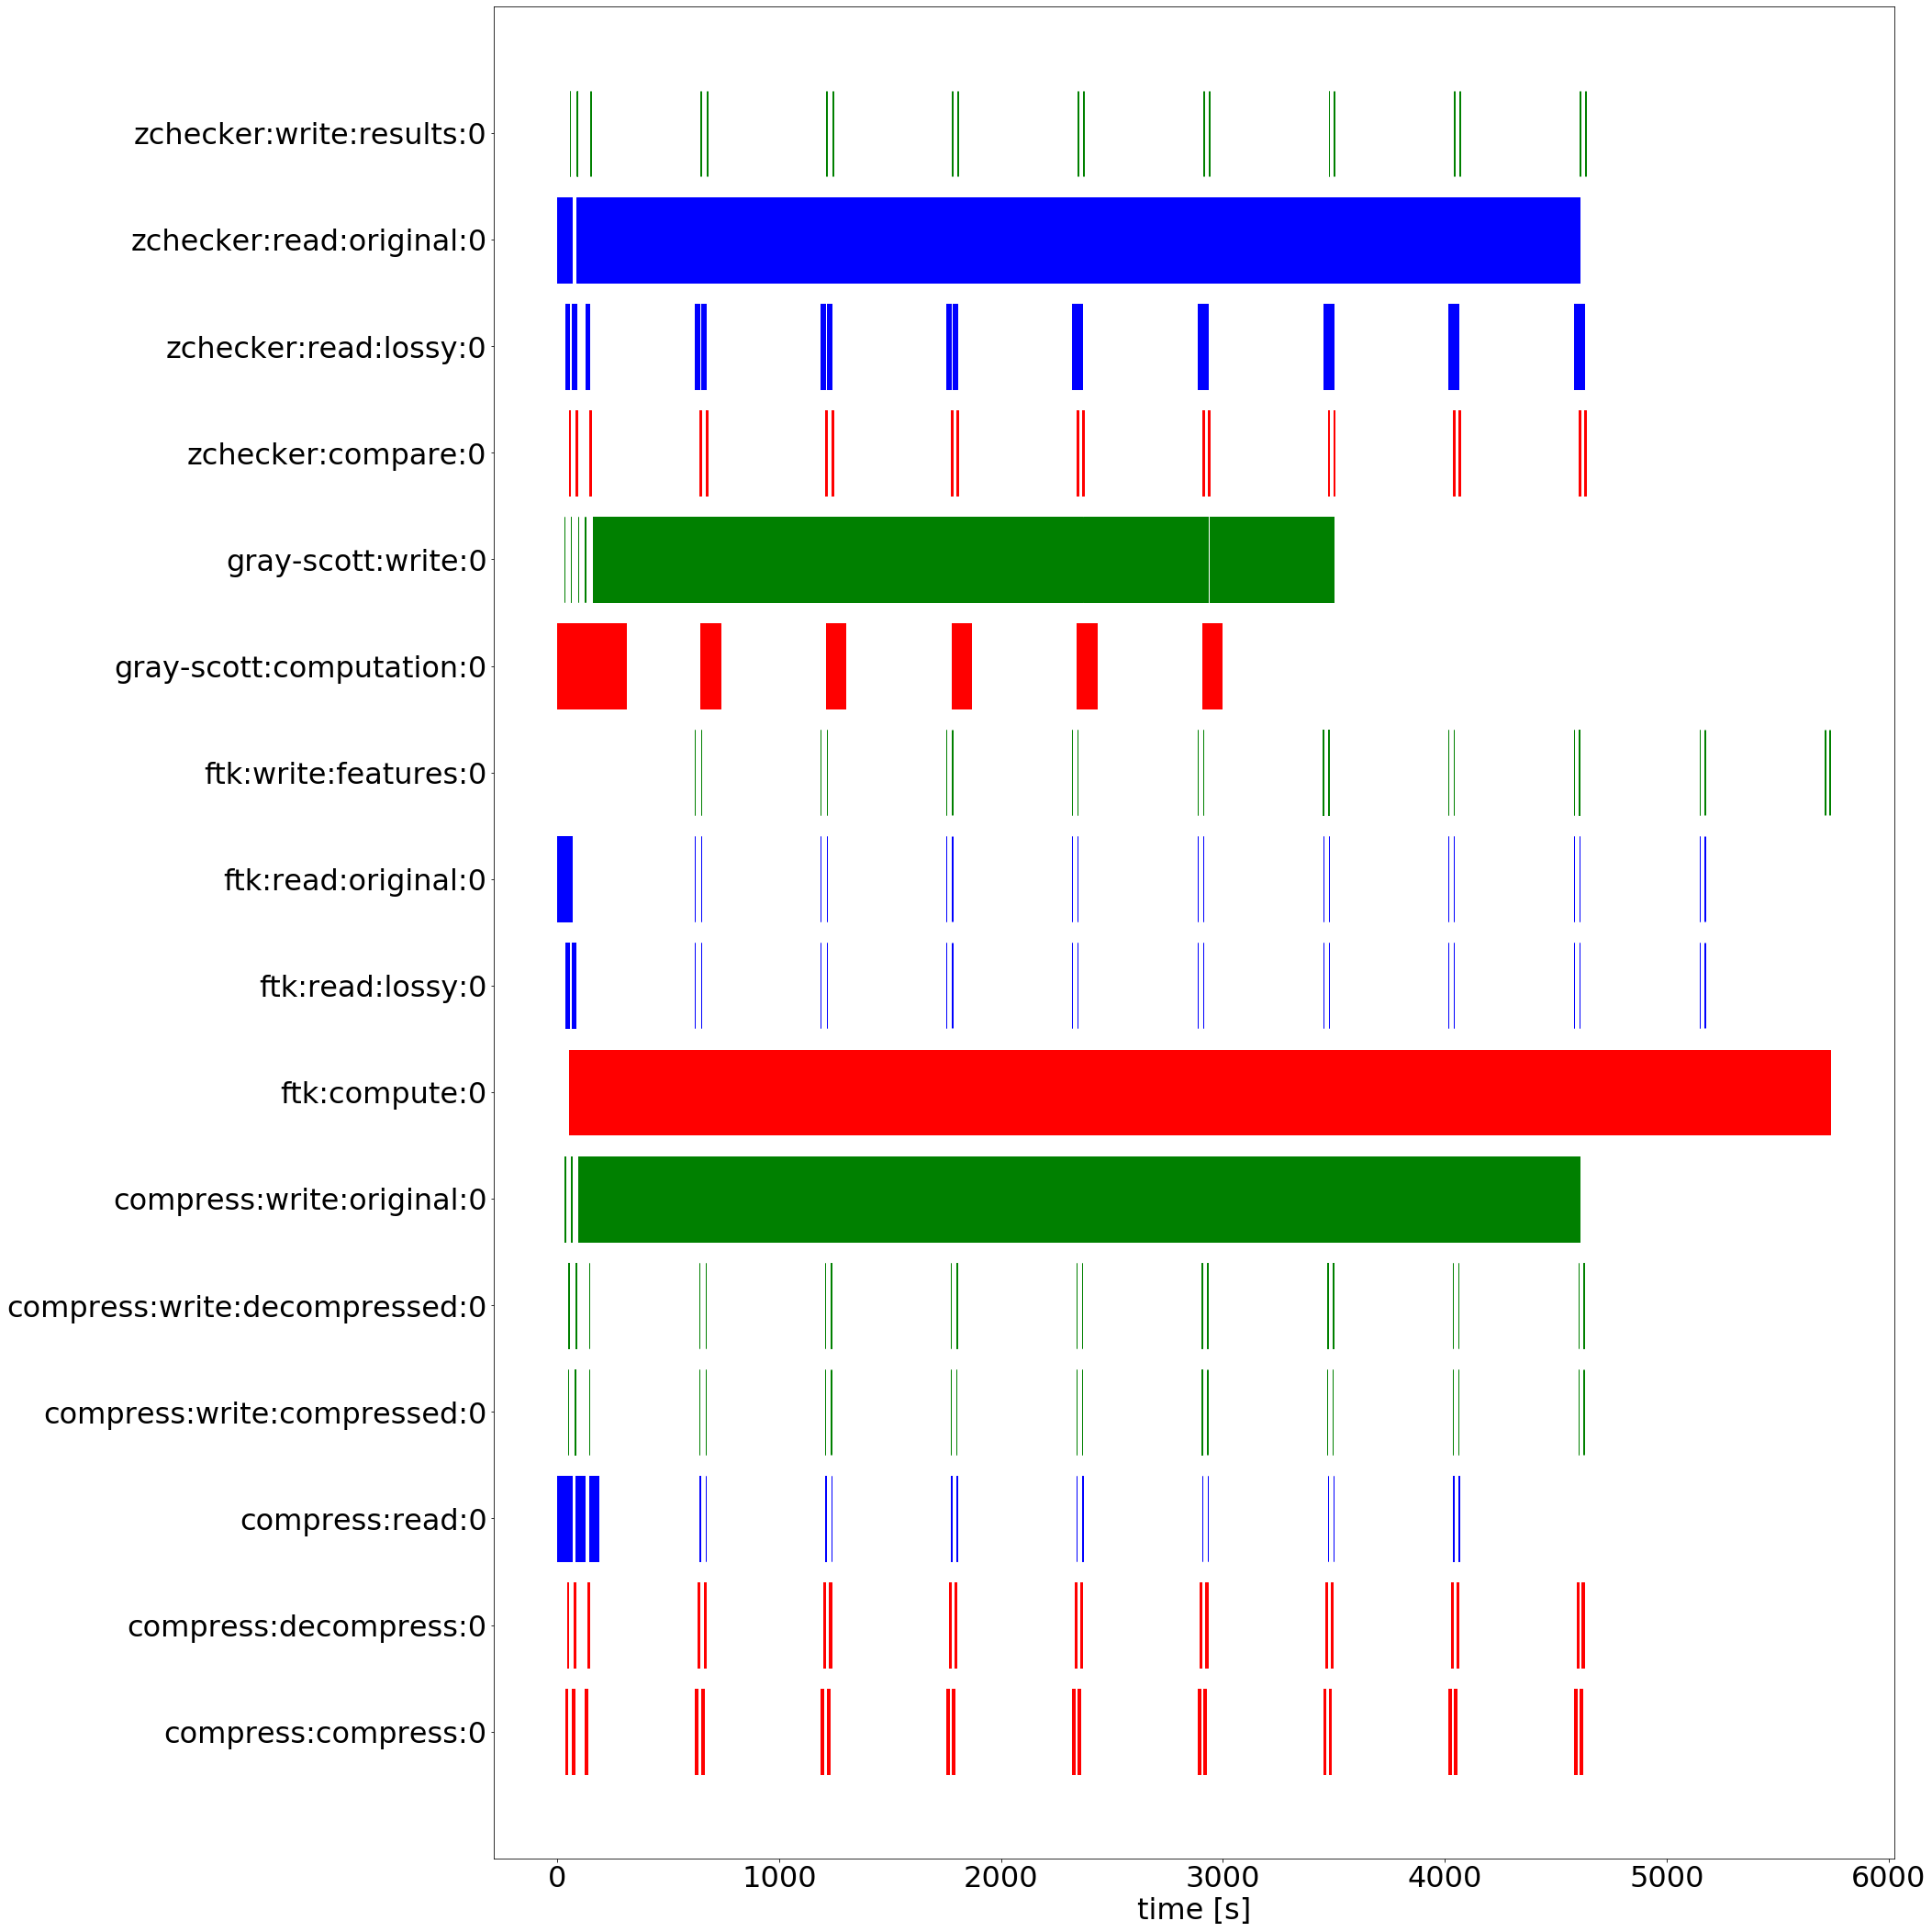
\includegraphics[width=8cm]{graphs/gantt_theta.png}
  \end{center}
\end{frame}


\begin{frame}[fragile]
  \frametitle{Gantt chart on Theta}
  \begin{itemize}
  \item Timing is shown for SZ, $U$, $256^3$ grid
  \item Only one MPI rank of each pipeline component is shown, other ranks have identical timing
  \item Red corresponds to computations: Gray-Scott compute, compression/decompression, ZChecker and FTK comparisons
  \item Green corresponds to write
  \item Blue corresponds to read
  \item Everything is dominated by FTK computations, all other computations take negligible time in comparison
  \item Long times for I/O are misleading. ADIOS2 SST streams are configured in such a way that
    \begin{itemize}
    \item Gray-Scott waits for compressor to pick up its checkpoint before proceeding to the next iteration
    \item compressor waits for ZChecker and FTK to pick up its data before proceeding to the next iteration
    \end{itemize}
  \item As a result, long I/O times are due to waiting for FTK to finish the previous iteration and not due to actually moving bits
  \end{itemize}
\end{frame}


\subsection{adios2.xml}
\begin{frame}[fragile]
  \frametitle{Gantt chart on Theta: adios2.xml}

  \begin{columns}

    \begin{column}{0.5\textwidth}
{\tiny
\begin{verbatim}
<adios-config>
 <io name="SimulationOutput">
  <engine type="SST">
  <parameter key="RendezvousReaderCount" value="1"/>
  <parameter key="QueueLimit" value="1"/>
  <parameter key="QueueFullPolicy" value="Block"/>
 </engine>
</io>
<io name="OriginalOutput">
 <engine type="SST">
  <parameter key="RendezvousReaderCount" value="2"/>
  <parameter key="QueueLimit" value="1"/>
  <parameter key="QueueFullPolicy" value="Block"/>
 </engine>
</io>
<io name="CompressedOutput">
 <engine type="BPFile">
  <parameter key="RendezvousReaderCount" value="1"/>
  <parameter key="QueueLimit" value="1"/>
  <parameter key="QueueFullPolicy" value="Block"/>
 </engine>
</io>
\end{verbatim}
}

    \end{column}

    \begin{column}{0.5\textwidth}

{\tiny
\begin{verbatim}
<io name="DecompressedOutput">
 <engine type="SST">
  <parameter key="RendezvousReaderCount" value="2"/>
  <parameter key="QueueLimit" value="1"/>
  <parameter key="QueueFullPolicy" value="Block"/>
</engine>
</io>
<io name="FTK">
 <engine type="BPFile">
  <parameter key="RendezvousReaderCount" value="1"/>
  <parameter key="QueueLimit" value="1"/>
  <parameter key="QueueFullPolicy" value="Block"/>
 </engine>
</io>
</adios-config>
\end{verbatim}
}
      
    \end{column}
  \end{columns}


\end{frame}




\subsection{Detailed comparison}
\begin{frame}[fragile]
  \frametitle{Detailed comparison}

{\tiny
\begin{table}[H]
\centering
\begin{tabular}{|r|r|r|r|r|r|}
\hline
 & \multicolumn{3}{|c|}{Summit} & \multicolumn{2}{|c|}{Theta} \\
 \hline	
	 & MPI ranks & CPU threads & GPUs & MPI ranks & CPU threads\\
\hline
	Gray-Scott & 2 & 1 & 2 & 64 & 1\\
\hline
	SZ & 1 & 1 & 0 & 1 & 1\\
\hline
	ZFP & 1 & 1 & 0 & 1 & 1\\
\hline
	MGARD & 1 & 1 & 0 & 1 & 1\\
\hline
	ZChecker & 5 & 1 & 0 & 64 & 1\\
\hline
	FTK & 1 & 20 & 0 & 1 & 64\\
\hline
\end{tabular}
\caption{Utilized computational resources}
\label{cresources}
\end{table}
}

{\tiny

\begin{table}[H]
\centering
\begin{tabular}{|r|r|r|}
\hline
	 & Summit & Theta\\
\hline
	Gray-Scott compute & $14 \pm 0.05$ & $32 \pm 0.2$ \\
\hline
	SZ compress & $2.5 \pm 0.05$ & $11 \pm 0.5$ \\
\hline
	SZ decompress  & $2.0 \pm 0.15$ & $ 7.9 \pm 0.5$ \\
\hline
	ZFP compress & $0.4 \pm 0.3 $ & $1.3 \pm 1.1$ \\
\hline
	ZFP decompress & $0.43 \pm 0.35$ & $1.5 \pm 1.2$ \\
\hline
	MGARD compress & $15 \pm 6$ & $72 \pm 48$\\
\hline
	MGARD decompress & $2.2 \pm 0.07$ & $16 \pm 0.7$\\
\hline
	ZChecker compare & $1.9 \pm 0.009$ & $3.5 \pm 0.1$ \\
\hline
	FTK compare & $81 \pm 0.3$ & $560 \pm 0.8$ \\
\hline
\end{tabular}
\caption{Average timing of various pipeline components in seconds.
  Grid size $256^3$. Gray-Scott simulation was run 1000 time steps, saving checkpoints every 100 iterations.
Therefore the averaging was done over 10 samples. The input compression tolerance here is fixed at $10^{-3}$. }
\label{timing}
\end{table}

}

  
\end{frame}


\begin{frame}[fragile]
  \frametitle{Detailed comparison}

  \begin{itemize}
  \item On Summit the whole pipeline fits into a single node
  \item On Theta each component runs on a separate node - 4 nodes

  \item Notice that timing for SZ compression/decompression is measured differently than for ZFP and MGARD:
    SZ times include both $U$ and $V$ variables, while for the other compression algorithms time is measured separately
    for different variables and this is the origin of high std for ZFP and MGARD and higher mean for SZ. This needs to be unified later.

  \item If instead of 64 hardware threads, one uses all 256 hardware threads on theta's KNL node,
    FTK compare time drops from $560$ to $480 \pm 0.6$ seconds.
  \item  If instead of 64 MPI ranks for Gray-Scott on Theta, one uses 32 MPI ranks,
    the run time for 100 iterations increases from $32$ to $62 \pm 0.3$ seconds.

  \item If instead of 64 MPI ranks for ZChecker comparison on theta, one uses 32 MPI ranks,
    the run time increases from $1.9$ to $7 \pm 0.2$ seconds.
  \end{itemize}
\end{frame}


\begin{frame}[fragile]
  \frametitle{Detailed comparison}
  \begin{itemize}
  \item FTK is the biggest bottleneck
  \item MGARD is much slower than other compression algorithms
  \item Theta is much slower than Summit
  \item Possible improvements to timing:
    \begin{itemize}
    \item FTK is called 4 times sequentially for original and lossy data, for $U$ and $V$ - this can be done in parallel using MPI;
      debugging the corresponding version
    \item Currently FTK can only use CPU threads - accelerate it to use GPUs
    \item Hanqi's summer students integrated FTK with MPI - might help on Theta but not on Summit
    \item Recent development in MGARD - it is cudarized now
    \end{itemize}
  \end{itemize}
\end{frame}
